\chapter{Ergebnisanalyse}

\todo{nochmal schauen ob Überleitung noch stimmt wenn Implementierungsteil geschrieben wurde...}
Nachdem im letzten Abschnitt ausführlich beschrieben wurde wie der komplette Komponentenstack im Detail implementiert wurde, werden im Folgenden auf die erhaltenen Metriken erläutert. Es wird insbesondere auf die Bedeutung einzelner Messwerte, sowie auf mögliche Begründungen dieser eingangen.


\todo{folgende Stichpunkte entfernen}
\begin{itemize}
  \item Latenzzeit im Durchschnitt sowie als zeitliche Historie
  \begin{itemize}
    \item Abschnitt \emph{vor} Datenaufnahme gesondert betrachten
    \item Abschnitt \emph{nach} Datenaufnahme gesondert betrachten
    \item Gesamte Pipeline betrachten
  \end{itemize}
  \item Skalierungsdauer jeweils pro verwendeter Backend-Technologie festzuhalten
  \begin{itemize}
    \item Skalierung anhand eingehender Nachrichten mittels Stufenmodell
    \item Skalierung mittels direkter Benutzeranfrage (ohne eingehende Nachrichten)
    \item Metriken als Datensätze in einer Datenbank hinterlegt
    \item Durchschnittliche Startzeit pro Containeranzahl 
    \item Durchschnittliche Startzeit pro Skalierungsstufe 
    \item Gesamtdurchschnittliche Startzeit als einzelner Messwert
    \item Metriken als zeitlicher visualisiert
  \end{itemize}
\end{itemize}




\section{Ergebnisse}
\begin{itemize}
  \item Vorstellung der erhaltenen Daten
  \item Interpretation / Analyse allerdings Teil vom naechsten Kapitel?
\end{itemize}

\subsection{Latenzzeit}
Die wichtigsten Messdaten bezüglich der Leistungsfähigkeit des Systems beziehen sich auf den Datendurchsatz beziehungsweise die entsprechende Latenzzeit. In der Tabelle \ref{tab:latency} wurden diese für die beiden betrachteten Backendtechnologien gegenübergestellt. Alle Angaben wurden in Millisekunden erfasst. Ein im System eingegangene Nachricht verweilt bei Bearbeitung durch einen Node.js Konsumenten im Schnitt 38 Sekunden, während sich dieser Wert bei Spring Boot auf über eine Minute beläuft. Diese Werte bilden lediglich einen Durchschnitt aller erhaltenen Metriken ab, eine genauere Aufteilung bezüglich des Zusammenhangs zu den Skalierungsgrößen erfolgt im nächsten Abschnitt (siehe \todo{Ref einfuegen}). Der Gesamtdurchschnitt setzt sich aus zwei Zeitangaben der Pipeline zusammen: 

\begin{enumerate}
  \item Den Nachrichteneingang: Diese Metrik beschreibt den Zeitraum zwischen erhaltener Anfrage im System und Acknowledgement durch die Konsumer-Komponente, dass die Nachricht nun bearbeitet wird. Sie beläuft sich bei der Node.js Komponente auf ungefähr 34 Sekunden und 58 Sekunden bei der Spring-Boot-Komponente. 
  \item Die Verarbeitungsdauer: Diese Metrik beschreibt den Zeitraum zwischen Acknowledgement durch den Konsumer, dass die Nachricht erhalten wurde, sowie dem Abspeichern des extrahierten Wertes durch den Konsumenten in der Datenbank. Dieser Werte beläuft sich bei beiden Implementierung auf etwas über drei Sekunden. Bei dieser Metrik liegt der Fokus allerdings auf dem minimalen Zeitunterschied im Millisekundenbereich, da in beide Implementierungen eine künstliche Verlangsamung (\emph{Sleep-Funktion}) eingebaut wurde um die erhaltenen Messwerte besser nachvollziehen zu können. Bei Node.js liegt die tatsächliche Verarbeitungsdauer bei 388 Millisekunden \emph{(total 3388)}, während sie bei Spring Boot bei 29 Millisekunden liegt \emph{(total 3029)}.
\end{enumerate}

\begin{table}[ht!]
	\centering
	\caption[Latenzzeit - Vergleich]{Gegenüberstellung der Latenzzeiten}
  \label{tab:latency}
  \hspace{5mm}
  \begin{tabular}{@{}lc@{}}
    \toprule
    Metrik & Dauer \\
    \midrule
    Node.js \\
    \hspace{3mm}Gesamtdurchschnitt & 38416 \\
    \hspace{3mm}Nachrichteneingang & 35027 \\
    \hspace{3mm}Verarbeitungsdauer & 3388 \\
    \midrule
    Spring Boot \\
    \hspace{3mm}Gesamtdurchschnitt & 61800 \\
    \hspace{3mm}Nachrichteneingang & 58771 \\
    \hspace{3mm}Verarbeitungsdauer & 3029 \\
    \bottomrule
  \end{tabular}
\end{table}


\subsection{Skalierungsdauer}
Diese Gruppe an Metriken bezieht sich auf die genauen Zeiträume, welche benötigt werden, um einen Container mit der entsprechenden Implementierung hochzufahren. 

\paragraph{Aufschlüsselung nach Containeranzahl}
Die grundlegendste Metrik beschreibt die Zeiten aufgeschlüsselt nach Anzahl gleichzeitig hochfahrender Container (siehe \ref{fig:specContainers}). Wie im Graphen erkennbar, handelt es sich um ein lineares Wachstum. Mit jedem zusätzlichen Container, der zeitgleich erstellt werden soll, dauert der Initialisierungsprozess bei der Spring-Implementierung im Schnitt 1611 Millisekunden länger. Bei der Node Implementierung liegt dieser Wert bei 194 Millisekunden. So dauert das Initialisieren eines einzelnen neuen Containers bei der Spring-Boot-Komponente 4,8 Sekunden während sich dieser Wert bei der Node.js-Koponente lediglich 2,6 Sekunden beläuft. Um diese nach Containeranzahl aufgeschlüsselten Werte zu erhalten, wurde nicht wie bei den anderen Skalierungstests auf die öffentliche Schnittstelle mittels Nachrichtengenerierung zurückgegriffen, es wurde stattdessen eine interne Schnittstelle mittels dediziertem Skript verwendet um möglichst Störungsfrei direkt auf die Komponente welche das Skalieren orchestriert zuzugreifen. Die nachfolgenden Metriken wurden allerdings durch die öffentliche Schnittstelle generiert.

\begin{figure}
  \centering
  \caption[Startzeit Container - Anzahl spezifisch]{Startzeit Container - Anzahl spezifisch}
  \label{fig:specContainers}
  \begin{tikzpicture}
    \begin{axis}[xlabel={Zusätzlich hochgefahrende Container}, ylabel={Startzeit}]
      \addplot table [x=additionalCnt, y=startupTime, col sep=comma] {kapitel/ergebnisanalyse/_data/springSpecificBenchmarks.csv};
      \addlegendentry{Spring Boot}
      \addplot table [x=additionalCnt, y=startupTime, col sep=comma] {kapitel/ergebnisanalyse/_data/nodeSpecificBenchmarks.csv};
      \addlegendentry{Node.js}
    \end{axis}
  \end{tikzpicture}
\end{figure}

\paragraph{Aufschlüsselung nach Skalierungsstufe}
Um einen beispielhaften Skalierngsalgorithmus zu implementieren wurde ein Regelsatz verfasst welcher vom Alert-Manager zur Laufzeit automatisch in einem festgelegten Interval ausgewertet wird. Um diesen Regelsatz zu Vorführungszwecken nicht unnötig ausführlich zu gestalten, wurde das Hinzufügen neuer Instanzen in Stufen organisiert. Im folgenden werden die Messwerte dieser Stufen näher erläutert. 



% \begin{tikzpicture}
 
  % \begin{axis} [xbar]
  % \addplot coordinates {
  %     (Nodejs,6610) 
  %     (Spring,35336)
  % };
  % \end{axis}
   
  % \end{tikzpicture}

% \begin{table}[ht]
%   \caption{Partial horizontal line}
%   \begin{tabular}{lll}
%       \hline
%       \multicolumn{2}{c}{Multi-column}&234234\\
%       \cline{1-2}
%       &Nachrichteneingang&213123\\
%       &Verarbeitungsdauer&324324\\
%       \hline
%   \end{tabular}
%   % \end{center}
%   \label{tab:multicol}
%   \end{table}


\begin{figure}
	\centering
	\caption[Startzeit Services]{Durchschnittliche Startzeit pro Service}
  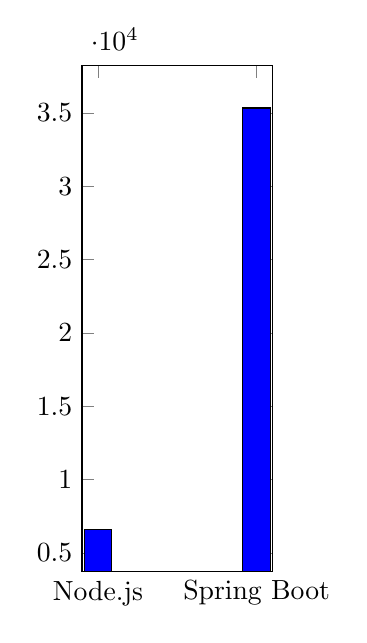
\begin{tikzpicture}
    \begin{axis}[
        symbolic x coords={Node.js,Spring Boot},
        width=4cm,
        height=8cm,
        xtick=data]
        \addplot[ybar,fill=blue] coordinates {
            (Node.js,6610)
            (Spring Boot,35336)
        };
    \end{axis}
  \end{tikzpicture}
\end{figure}

\begin{figure}
	\centering
	\caption[Startzeit Stufenübersicht]{Durchschnittliche Startzeit stufenweise - Node}
  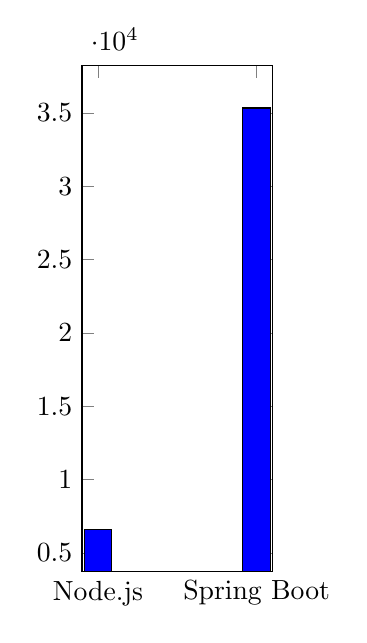
\begin{tikzpicture}
    \begin{axis}[
        symbolic x coords={Node.js,Spring Boot},
        width=4cm,
        height=8cm,
        xtick=data]
        \addplot[ybar,fill=blue] coordinates {
            (Node.js,6610)
            (Spring Boot,35336)
        };
    \end{axis}
  \end{tikzpicture}
\end{figure}




% \begin{tikzpicture}
%   \begin{axis}[
%       coords={Nodejs, Spring Boot},
%       xtick=data,
%       width=3cm,
%       height=5cm
%     ]
%       \addplot[ybar,fill=blue] coordinates {
%           (Nodejs,      6610)
%           (Spring Boot,  35336)
%       };
%   \end{axis}
% \end{tikzpicture}

% \begin{figure}
%   \begin{tikzpicture}
%     \begin{axis}[
%       mbarplot,
%       ymin = 0,
%       ymax = 1,
%       xlabel={},
%       ylabel={},
%       width=0.9\textwidth,
%       height=7cm,
%       xtick=data,
%       symbolic x coords={KNN,E1,E2,E3,E4}
%     ]
%       \addplot table [x=serviceName, y=averageStartupTime, col sep=comma] {kapitel/ergebnisanalyse/_data/nodeSpecificBenchmarks.csv};
%       \legend{Service Startzeit - Durchschnitt}

%     \end{axis}
%   \end{tikzpicture}
% \end{figure}






\section{Analyse}
\begin{itemize}
  \item Interpretation / Analyse der Daten
  \item Begruendung fuer Verhalten suchen
\end{itemize}

\section{Diskussion}

\subsection{Begr\"undung Startupzeit}
\begin{itemize}
  \item Warum Node.js schneller ist
\end{itemize}

\begin{itemize}
  \item Erlaeutern warum die erhaltenen Ergebnisse in einem real-life Szenario vielleicht nicht aussagekraeftig sein koennten
\end{itemize}
